% !TEX root = thesis.tex

\section{Els moviments de Reidemeister}\label{sec:Reidermeister}
Una primera aproximació per tal de distingir si dos nusos son diferent és veure quan son iguals. Aquesta és la inspiració darrera de la següent secció que tractarà sobre els moviments de Reidemeister i el Teorema central de la Teoria de Nusos.

\subsection{Moviments de Reidemeister}\label{subsec:Moviments de Reidemeister}
Motivats per la Secció \ref{Equivalència entre nusos}, un podria veure sense massa dificultat que cadascun dels moviments de la Figura \ref{fig:Moviments de Reidemeister} resulta en un diagrama de nus equivalent a l'original.\\

\begin{figure}[h]
	\centering
	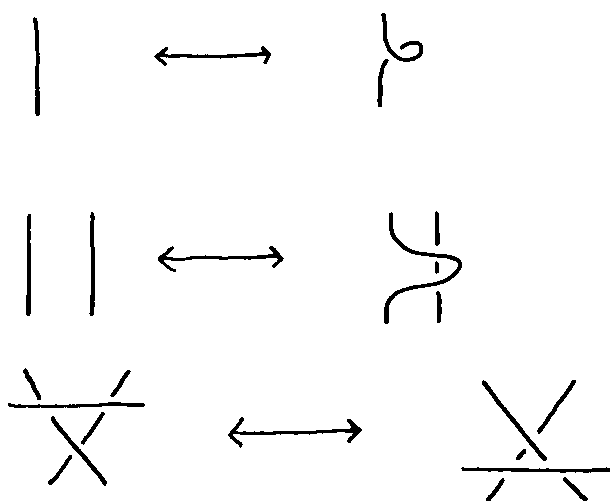
\includegraphics[width=0.9\linewidth]{img/MovimentsdeReidemeister.png}
	\caption{De dalt a baix: Moviment de Tipus I, Tipus II i Tipus III  [\cite{SobreelsmovdeReide}]. Cal pensar que els segments lliures de corda s'uneixen a través d'un nus $K$.}\label{fig:Moviments de Reidemeister}
\end{figure}

A aquests tres tipus de moviments se'ls anomena moviments de Reidemeister. Al primer de tots se'l diu de Tipus I o \textit{twist} en anglès, al segon de Tipus II o \textit{poke} i al tercer de Tipus III o \textit{slide}.\\

\noindent
\textbf{Moviment de Tipus I o \textit{twist}:} També anomenat \textbf{RI} per abreujar notació, aquest tipus de moviment consisteix en "pessigar" la corda i amb el tros obtingut donar-li la volta (d'aquí el nom en anglès) fent un bucle com en el de la Figura \ref{fig:Moviments de Reidemeister}.\\

\noindent
\textbf{Moviment de Tipus II o \textit{poke}:} També anomenat \textbf{RII}. Aquest tipus de moviment consisteix en fer passar una de les dues cordes per sobre de l'altra. En anglès, la paraula \textit{poke} significa fer passar forçosament alguna cosa en una certa direcció i doncs en aquest cas es podria pensar que una de les dues cordes s'ha fet passar per sobre de l'altra.\\

\noindent
\textbf{Moviment de Tipus III o \textit{slide}:} També anomenat \textbf{RIII}. Aquest tipus de moviment consisteix en, com el nom en anglès indica, fer lliscar una de les tres cordes d'una banda a l'altra de la intersecció entre les dues cordes restants. En la Figura \ref{fig:Moviments de Reidemeister} podem veure com el segment de corda horitzontal llisca de dalt a baix del creuament entre les altres dues cordes.\\

Continuant amb el que hem vist, no és massa difícil veure que aplicant una seqüència finita de moviments RI, RII o RIII a un diagrama de nus qualsevol, el nus obtingut és equivalent a l'original.

\subsection{El Teorema central de la Teoria de Nusos}\label{sec:teoremacentraldelateoria}

L'any 1930, Kurt Reidemeister demostrà que l'implicació contrària també és certa, és a dir que si dos diagrames de nusos qualssevol son equivalents, aleshores sempre podem trobar una seqüència finita de moviments de Reidemeister de manera que podem transformar un diagrama de nus en l'altre. Aquest resultat va donar lloc al teorema central de la teoria.

\begin{theorem}\label{teo:teoremadeReidemeister}
   $diag(K)$ i $diag(K')$ son equivalents si i només si, existeix una seqüència finita de moviments RI, RII o RIII que passa d'un a l'altre.
\end{theorem}

Una demostració del teorema original es pot trobar a (Knot Knotes Justin Roberts, pàgina 18 Teorema 2.3.1) \cite{knotentheorie}, \textbf{però en essència aquesta demostració fa ús del fet que la manera en que un pot generar nusos equivalents a l'original és a través d'afegir triangles als costats d'un nus poligonal.}\\

\begin{figure}[H]
	\centering
	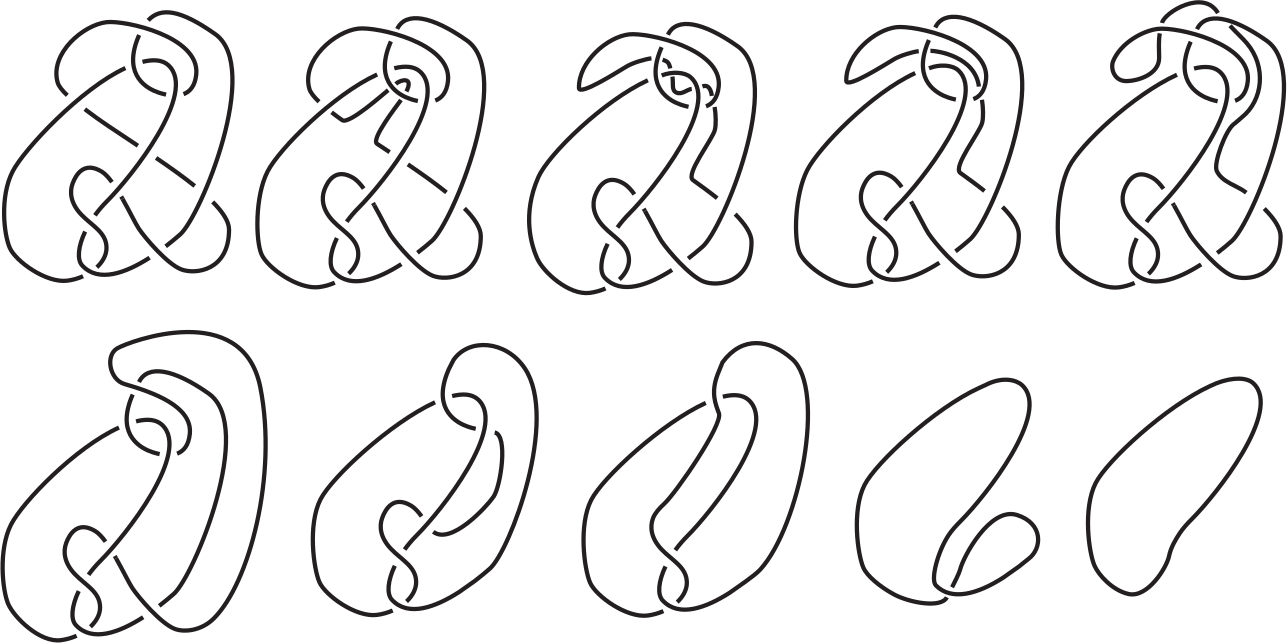
\includegraphics[width=0.9\linewidth]{img/culprit-knot.png}
	\caption{Com es pot observar en l'exemple, el nus de Culprit és equivalent al nus zero o \textit{unknot} en anglès. Mitjançant la seqüència de moviments següent podem passar de l'un a l'altra. D'esquerra a dreta i de dalt a baix: RII, RIII+RIII, RII, RIII, RI+RII, RII, RII, RII, RI, [\cite{culpritknot}].}\label{fig:culpritknot}
\end{figure}

El Teorema \ref{teo:teoremadeReidemeister} doncs, posa en evidència el fet que parlar d'equivalència entre nusos o d'equivalència entre diagrames de nusos és el mateix, doncs aquests estan en correspondència a través de la Secció \ref{sec:Representació de nus}.\\

D'aquesta manera i fent referència al mencionat anteriorment, a partir d'ara farem un abús de llenguatge i notació dient nus $K$ indistintament sense posar importància al fet de si ens referim al nus o al seu diagrama.